As robotic applications flourish in our modern world, there is an increasing need for  high reduction, high torque, and low backlash actuator systems.
These actuators are present in all types of robotic equipment and are critical in space flight applications as well.
A notable recent example includes the Curiosity rover from NASA's Jet Propulsion Laboratory that uses 33 separate motors with various reductions \cite{curiosity}.
Currently, harmonic drives are the primary reduction method when high ratio and compact design are required.
These reducers come in limited reduction ratio options, and can grown quite heavy to withstand the high torque applications.
Ideally, one would be able to specify a desired reduction ratio and realize it in a compact, lightweight package.

\subsection{Cycloidal Drive Motivation}

Cycloidal drives are potentially an apt replacement for these harmonic drives as they can offer large a large reduction in a small package.
In situations where small backlash is acceptable, cycloids offer distinct advantages.
They can be customized into the system directly and are made of relatively easy to manufacture parts.
In addition, the torque to weight ratio typically higher for cycloidal drives of this style.
For example, the cycloid presented in this work is 2.5kg, including all housing components while a comparable harmonic drive is 5.1kg.
Despite these desirable features, there is insufficient data available to quantify the true efficiency and characteristics of these drives.

The primary contribution of this research is to quantify the efficiency of a cycloidal drive system through an extended drive cycle test for burn-in to steady state performance over 51K output revolutions through over 100 hours and efficiency testing over the torque and speed range of this system.

\begin{figure}[!b]
   \centering
   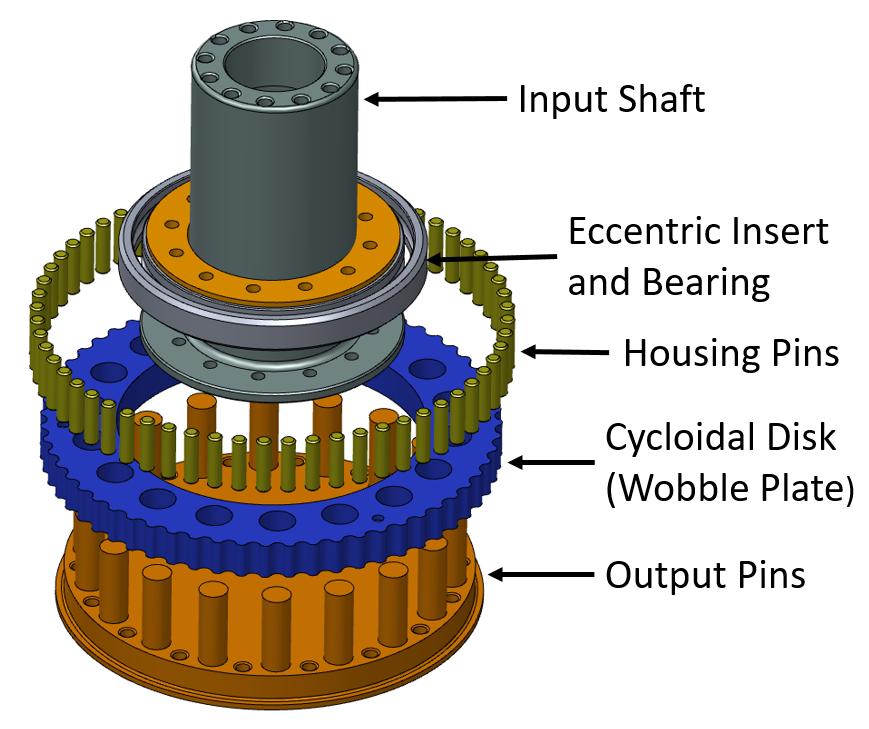
\includegraphics[width=0.50\linewidth]{images/cycloid_cartoon_v2}
   \caption{Simple rendering of the key elements that create a cycloidal drive.
   A drive shaft spins a cycloidal disk (wobble plate) via an eccentric circle.
   The wobble plate reacts against the housing pins to create a counter-rotation, harnessed by the output pins.}
   \label{cycloid_cartoon}
\end{figure}

\subsection{Cycloidal Drive Background}
Cycloidal drives were proposed as early as 1956 by Botsiber and Kingston \cite{1956}.
The premise of this design leverages a plate, referred to as the wobble plate, with lobes interacting with pins in the housing designed using trochoidal motion being spun on an eccentric shaft with a bearing.
This induces a counter-clockwise motion of the plate that is harnessed with the interior pins as the output of the mechanism (seen in Fig \ref{cycloid_cartoon}).
This geartrain design has been used in industry for high torque, high shock load applications for many years including companies like Natbesco Motion Control.
However, in many of these applications, all of the interacting surfaces like the housing pins and output pins use needle roller bearings to transmit load.
This allows for higher efficiency and load carrying capability, but it also increases mass and volume.
In the robotic industry, groups are striving to reduce the mass and volume of these actuators while still achieving  high reduction and load capabilities, by eliminating many of the rolling elements at the interaction points between the wobble plate, housing pins, and output pins.
This allows for very compact and strong designs to be considered, but leaves the potential for larger losses and shorter system lifetime.


Many works have been presented on the subject of the theoretical design of these cycloidal drives \cite{on_the_lobe} \cite{hwang_hsieh}, designing with machine tolerances \cite{design_and_application}, contact and stress analysis \cite{li}, and performance characteristics such as torque ripple and backlash \cite{hsieh_traditional} \cite{hsieh_dynamics} as will be presented in Section \ref{design}.
These works lay a solid foundation for a designer, providing the equations and design considerations for a cycloid.
Still, there is a need to present in-use characteristics to support the theoretical calculations and models.


Theoretical cycloid efficiencies have been reported in the 88-98\% range \cite{Malhorta}, \cite{unified_approach}.
More recently, Sinsinger and Lipsey reported experimentally determined efficiencies for fused roller designs (42.3\%) and pin designs (71\%) based on 80 minutes of run-time \cite{cycloid_vs_harmonic}.
The distinction between a fused roller and pin design comes in the design of the housing.
In a fused design, the housing lobes are part of the housing, and in a pin design, pins are inserted the ride in the housing, allowing relative motion.

Hsieh verified the stress present in the drives in simulation and in use and demonstrated lower stress levels and torque ripple when using fused rollers \cite{hsieh_dynamics}.

These two results leave an open trade to designers if stress and torque ripple need to be minimized versus efficiency maximized.

The aim of this work is to utilize a custom cycloid design for a NASA rover application and show the in-use efficiency characteristics over an extended duration test.
The actuator design is presented in Section \ref{design}.
A description of the experimental setup and procedure is provided in Section \ref{methods}.
Finally, the results and analysis of this high torque actuator and its implications are presented and discussed in Section \ref{results} and Section \ref{discussion}.

